\vspace{-0.05in}
\section{Simulation Studies}\label{sec_simulation}
\vspace{-0.05in}

We demonstrate the accuracy of our results in simulations.
While our theory is asymptotic (with error terms that are negligible when $p$ is sufficiently large), we observe that they are incredibly accurate in a moderate dimension of $p = 200$.

\textbf{Sample efficiency.}
First, we validate the result of Example \ref{ex_same_cov}.
Figure \ref{fig_same_cov} shows the average prediction loss over ten tasks as we increase the number of samples per-task from $400$ to $2000$.
In all the parameter settings, our results estimate the empirical losses accurately.
We also observe a trend that the average prediction loss increases as we increase distance $d$ from $0.1$ to $0.2$.
Our work explains the differences between these two settings since $d^2 = 0.1^2$ is always smaller than $\frac{\sigma^2 p}{n - p}$, but $d^2 = 0.2^2$ is not.
%Second, when $d = 0.1$, we have that $d^2 \le \frac{\sigma^2 p}{n - p}$ for all values of $n$, hence the average prediction loss of hard parameter sharing is always lower than STL.
Indeed, we observe a crossover point between hard parameter sharing and STL.
Finally, for $d = 0.2$, looking horizontally, we find that HPS requires fewer samples per-task than STL to achieve the same loss level. %\FY{I do not quite understand this sentence about "3x fewer", because how much data needed depends on $d$ and the prediction loss level we are looking at. For example, at the cross point, this ratio is 1. }

\textbf{Sample size ratio.}
Second, we validate the result of Example \ref{ex_sample_ratio}.
Figure \ref{fig_size} shows task two's prediction loss  as we increase the sample ratio $n_1 / n_2$ from $1/10$ to $7/10$.
%Again, our estimates are accurate compared to the empirical losses.
We consider a regime where task two consists of $80,000$ samples, and task one's sample size varies from $8,000$ to $56,000$. 
The task-specific variance (which scales with model distance) is $d = 0.2$, the noise variance is $\sigma^2 = 4^2$, and the shared signal variance is $1$. We observe that as we increase the sample ratio, task two's prediction loss decreases initially but later will increase when the sample ratio is above a certain level.
On the other hand, when $d = 0.15$, task two's prediction loss decreases faster.
Intuitively, this is because bias increases less for smaller $d^2$.
%Our result from Corollary \ref{cor_MTL_loss} explains this trend.

\textbf{Covariate shift.}
Finally, we validate the result of Example \ref{ex_covshift}.
Figure \ref{fig_covariate} shows task two's prediction loss as we increase task one's sample size.
Recall that $\lambda$ measures the severity of covariate shifts---a larger $\lambda$ means a larger covariate shift.
We indeed observe the dichotomy in Example \ref{ex_covshift} at $n_1 = 800$.
The sample size $n_2$ is $800$ and the noise variance $\sigma^2$ is $1/4$.
%Covariate shift: We set $\kappa = 1$ and $d = 0$.
%We set $\rho_2 = 4$ and vary $\rho_1$ from $5$ to $25$ for sample sizes.
%We use the scale parameter $\lambda = 1$ for the curve without covariate shift and $\lambda = 2$ for the curve with covariate shift (cf. Section \ref{sec_covshift}).


%Recall that Section \ref{sec_data_size} shows that increasing the data size of the source task does not always improve the performance of MTL for the target task.
%In Figure \ref{fig_ab_data}, we show that for source task MR and target task SST, there is a transition from positive to negative transfer as we increase the data size of the source task.
%Our result provides a fine-grained insight on the covariance alignment algorithm proposed in \cite{WZR20}.
%Recall that the covariance alignment procedure in \cite{WZR20} adds an additional module between the word embedding representation and the shared module.
%When the source task data size is particularly large compared to the target task, we show that applying the covariance alignment algorithm results in more significant gains.
%In Figure \ref{fig_ab_cov}, we observe that the benefit from aligning task covariances becomes more significant for LSTM and MLP as we increase the number of datapoints of the source task.

%\begin{table}
%	\begin{center}
%		\begin{tabular}{c c c c c}
%			\toprule
%			\multirow{2}{*}{{\bf Models}} & \multicolumn{2}{c}{\begin{minipage}{1.1in}\begin{center}
%				                                                                          MR, SST, SUBJ, CR, MPQA, TREC\end{center}\end{minipage}} & \multicolumn{2}{c}{\begin{minipage}{1.1in}\begin{center}MR, SST, SUBJ, CR, MPQA\end{center}\end{minipage}} \\
%			\cmidrule(lr){2-3} \cmidrule(lr){4-5}
%			& {\bf Stanford} & {\bf Alignment} & {\bf Stanford} & {\bf Alignment} \\
%			\midrule
%			{\bf MLP}  & > 100\% & 39\% & 25\% & 25\% \\
%			{\bf LSTM} & 36\% & 36\% & 28\% & 25\% \\
			% {\bf CNN}  & 76\% & - & 32\% & -\\
%			\bottomrule
%		\end{tabular}
%	\end{center}
%	\caption{Taskonomy experiment.}
%	\label{tab:taskonomy}
%\end{table}
%\begin{figure}[!t]
%	\centering
%	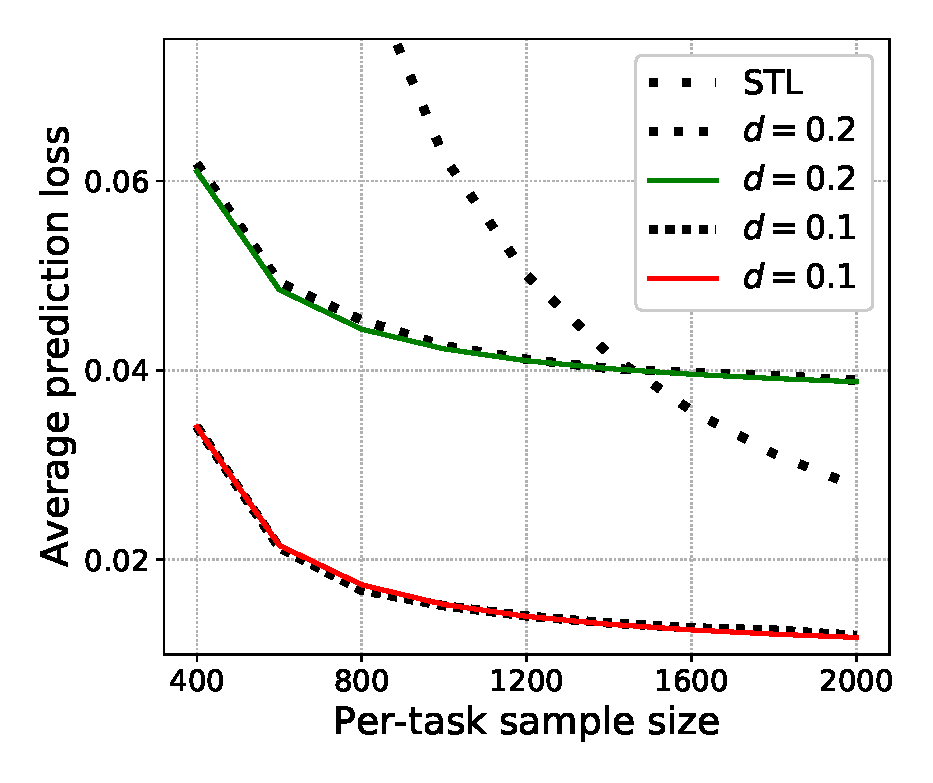
\includegraphics[width=0.35\textwidth]{figures/same_covariates.eps}
%	\caption{Validating Example \ref{ex_same_cov} in Section \ref{sec_same} for $10$ tasks: our estimated loss (solid line) matches the empirical loss (dotted line) accurately for various task-specific variance $d^2$ and sample size $n$ settings. The feature dimension $p$ is $200$, and noise variance $\sigma^2$ is $1/4$.}
%	\label{fig_same_cov}
%\end{figure}


